\section{Teoretická predpríprava}
\label{teoreticka predpriprava}

\subsection{Logistická regresia}
 
Logistická regresia je štatistická metóda využívaná pri binárnej klasifikácii.
Cieľom logistickej regresie je modelovať pravdepodobnosť nejakej triedy alebo udalosti (vysvetľovanej premennej)
na základe jednej alebo viacerých vysvetľujúcich premenných. TODO

Pred tým, než opíšeme, ako presne logistická regresia funguje, si zadefinujme niekoľko dôležitých pojmov, s ktorými logistická regresia narába.

\begin{defin}
    Logistická funkcia \( \sigma : \mathbb{R} \rightarrow (0, 1) \) je definovaná ako:
    \[
        \sigma(t) = \frac{e^t}{e^t + 1} = \frac{1}{1 + e^{-t}}
    \]
    Inverzná funkcia k logistickej sa nazýva logit funkcia a spĺňa:
    \[
        logit(t) = \sigma^{-1}(t) = \ln\left(\frac{p}{1 - p}\right)
    \]
    pre \( p \in (0, 1) \).
\end{defin}

Na obrázku je zobrazený graf logistickej funkcie na intervale \( (-6, 6) \):

% \begin{center}
%     \begin{tikzpicture}
%     \begin{axis}[
%         xlabel={x},
%         ylabel={y},
%         xmin=-6, xmax=6,
%         ymin=0, ymax=1,
%         xtick={-4,-2,0,2,4},
%         ytick={0,0.2,0.4,0.6,0.8,1},
%         legend pos=north west,
%         ymajorgrids=true,
%         grid style=dashed,
%         height=8cm,
%         width=15cm,
%     ]
    
%     \addplot[
%         color=blue,
%         mark=square,
%         ]
%         coordinates {
%         (2, 1.0)(3, 0.5)(4, 0.25)(5, 0.16667)(6, 0.11111)(7, 0.08333)(8, 0.0625)(9, 0.05)(10, 0.04)(11, 0.03333)(12, 0.02778)(13, 0.02381)(14, 0.02041)(15, 0.01786)(16, 0.015625)
%         };
%         % \legend{Rozptyl}
        
%     \end{axis}
%     \end{tikzpicture}
% \end{center}


\begin{center}
\begin{tikzpicture}[>=stealth]
    \begin{axis}[
        xmin=-6,xmax=6,
        ymin=0,ymax=1,
        axis x line=middle,
        axis y line=middle,
        axis line style=<->,
        xlabel={$x$},
        ylabel={$y$},
        ]
        \addplot[no marks,blue,solid] expression[domain=-6:6,samples=100]{1/(1 + exp(-x))};
    \end{axis}
\end{tikzpicture}
\end{center}

Argumentom prirodzeného logaritmu v logit funkcii je výraz \( \frac{p}{1 - p} \) pre \( p \in (0, 1) \).
Ak takéto \(p\) budeme chápať ako pravdepodobnosť, výraz \( \frac{p}{1 - p} \) predstavuje takzvaný pomer šancí (\emph{angl. odds-ratio}).
Napríklad pri hode kockou je pravdepodobnosť padnutia šestky rovná \( 1/6 \) a pomer šancí je \( \frac{\frac{1}{6}}{1 - \frac{1}{6}} = \frac{\frac{1}{6}}{\frac{5}{6}} = \frac{1}{5} = 1 : 5\),
čo znamená, že 1 možný výsledok hodu kockou zodpovedá šestke a 5 možných výsledkov šestke nezodpovedá.

Nech \( Y \) je binárna vysvetľovaná premenná, ktorej zodpovedá vektor vysvetľujúcich premenných \( x = (x_1, x_2, \ldots, x_k) \).
Pre \( Y \) zjavne platí \( P(Y = 1|x) = 1 - P(Y = 0|x) \).
Logistická regresia predpokladá, že logaritmus pomeru šancí (\emph{angl. log-likelihood ratio}) možno modelovať ako lineárnu funkciu zložiek vektora \( x \).

\[
\ln \left( \frac{P(Y = 1|x)}{P(Y = 0|x)} \right) = \ln \left( \frac{P(Y = 1|x)}{1 - P(Y = 1|x)} \right) = \beta_0 + \beta^T x
\]

Po úpravách sa ľahko dopracujeme k záveru, že pravdepodobnosť \( P(Y = 1|x) \) je rovná výstupu logistickej funkcie, ktorej argument bude hľadaná lineárna kombinácia zložiek vektora \( x \).

\begin{equation} \label{logistic_regression}
P(Y = 1|x) = \frac{1}{1 - e^{-(\beta_0 + \beta^T x})} := h(x)
\end{equation}

Ak logistickú regresiu používame na predikciu (čo budeme robiť neskôr v tejto práci),
vzorec (\ref{logistic_regression}) nám poslúži na výpočet pravdepodobnosti \( P(Y = 1|x) \) pri danom novom \( x \).

\subsubsection{Odhad parametrov v logistickej regresii}

Majme teda zovšebecnený regresný model tvaru

\[
h_\beta(x) = P(Y = 1|x) = \frac{1}{1 - e^{-(\beta_0 + \beta^T x})}
\]

Neznámymi parametrami v tomto modeli sú regresory \( \beta = (\beta_1, \ldots, \beta_k) \).
Na odhad regresných koeficientov sa vo väčšine prípadov používa metóda maximálnej vierohodnosti.
Na rozdiel od obyčajnej lineárnej regresie s normálne rozdelenými chybami, v logistickej regresii nie je možné nájsť exaktné vyjadrenie parametrov \( \beta \),
a na ich odhad sa používa nejaká iteračná metóda.

Keďže \(Y\) nadobúda len hodnoty z \( \{0, 1\} \), pre distribučnú funkciu \(Y\) platí:

\[
P(y | x; \beta ) = h_\beta(x)^y (1 - h_\beta(x))^{1 - y}
\]

Majme namerané vektory dát \( x_1, \ldots, x_n \), \( x_i = x_{i1}, \ldots, x_{ik} \),
a k nim prislúchajúce \( y_1, \ldots, y_n \). Potom pre funkciu vierohodnosti parametra \( \beta \) platí

\[
L(\beta | y; ) TODO
\]

Trénovanie logistickej regresie spočíva v maximalizovaní funkcie vierohodnosti,
čo je ekvivalentné maximalizácii jej logaritmu (\emph{angl. log-likelihood function}), a teda hľadáme

\[
TODO
\]

Na nájdenie maxima log-likelihood funkcie sa používajú iteračné metódy,
napr. funkcia \emph{glm} v základnej verzii jazyka \emph{R} využíva metódu \emph{IRLS} (\emph{iteratively reweighted least squares}).

\subsubsection{Sumárne štatistiky v logistickej regresii}

TODO: Tu napíšem niečo o hodnotách ako \(R^2\) atď., ešte to nemám celkom premyslené.

\subsubsection{Interpretácia parametrov v logistickej regresii}

TODO

\subsection{Bayesian averaging of classical estimates (BACE)}

Dáta, ktoré budeme spracúvať v našej práci, obsahujú 70 vysvetľujúcich premenných pre každý rok pôsobenia firmy.
Prirodzene, nie všetky z nich sa hodia na modelovanie bankrotu.
Naším cieľom bude vytvoriť model, ktorý bude relatívne jednoduchý, a v ktorom budú vystupovať len tie najsignifikantnejšie vysvetľujúce premenné z hľadiska predikcie bankrotu.
V tejto časti si opíšeme jednu z metód, ktorú použijeme, a to \emph{bayesian averaging of classical estimates} (\emph{BACE}).

Základná metóda \emph{BACE} bola vybudovaná za účelom vytvorenia lineárnej regresie, ale jej hlavnú ideu možno ľahko využiť aj pri logistickej regresii.
Názov \emph{bayesian averaging of classical estimates} vznikol na základe toho, že metóda BACE využíva bayesovské priemerovanie modelov (\emph{angl. bayesian averaging}) a klasické odhady parametrov lineárnej regresie metódou najmenších štvorcov.

\subsubsection{Bayesovská štatistika}

Metóda \emph{BACE} narába s teóriou bayesovskej štatistiky.
V klasickej štatistike predpokladáme, že parametre majú pevnú, ale neznámu hodnotu.
Neznáme parametre v klasickej štatistike nie sú náhodnými premennými a nemajú pravdepodobnostnú hustotu.
Narozdiel od toho v bayesovskej štatistike považujeme parametre za náhodné premenné, pričom ich náhodnosť zodpovedá miere neistoty, ktorú o danom parametri máme.

\subsubsection{Bayesovské priemerovanie modelov (bayesian model averaging)}

Jedným zo základných tvrdení bayesovskej štatistiky je tzv. bayesovo pravidlo, ktoré hovorí nasledovne:

\[
P(A|B) = \frac{P(B|A) P(A)}{P(B)}.
\]

Bayesovo pravidlo možno zovšeobecniť pre spojité náhodné premenné a ich hustoty. Pre náhodné premenné \(y\) a \( \beta \) platí:

\begin{equation} \label{bayes_rule}
    g(\beta | y) = \frac{f(y | \beta) g(\beta)}{f(y)}.
\end{equation}

Aplikujme vzorec (\ref{bayes_rule}) na premenné, ktoré vystupujú v logistickej regresii.
\( \beta \) je vektor parametrov (intercept a koeficienty jednotlivých vysvetľujúcich premenných),
\( g(\beta) \) je jeho apriórna hustota, ktorú interpretujeme ako presvedčenie výskumníka o parametri \( \beta \) predtým, než spoznáme dáta.
\( y \) je vektor nameraných dát, \( f(y) \) je jeho hustota.
\( g(\beta | y) \) je aposteriórna hustota parametra \( \beta \) (hustota podmienená nameranými dátami \( y \)) a predstavuje presvedčenie výskumníka o parametri \( \beta \) po tom, ako spoznáme dáta \( y \).
Bayesovo pravidlo hovorí o tom, ako skombinovať apriórnu informáciu \( g \) s nameranými dátami \( y \) a spočítať naše konečné presvedčenie o parametri \( \beta \) – jeho aposteriórnu hustotu \( g(\beta|y) \).

Majme množinu \( X = \{X_1, \ldots X_k\} \) potenciálnych vysvetľujúcich premenných pre model logistickej regresie.
Pri skúmaní signifikantnosti jednotlivých premenných \( X_1, \ldots, X_k \) máme možnosť danú premennú do modelu zaradiť alebo nezaradiť,
existuje teda celkovo \( 2^k \) modelov so všetkými možnými kombináciami parametrov \( X_1, \ldots, X_k \).
(\( M_i \) môže byť reprezentované napr. binárnym vektorom dĺžky \(k\), pričom hodnota na mieste \( j = 1, \ldots, k \) hovorí o zaradení, resp. nezaradení \(j\)-tej vysvetľujúcej premennej do modelu.)

Výskumník zvolí apriórne pravdepodobnosti \( p(M_i) \), pričom \( \sum p(M_i) = 1 \) (problematikou voľby apriórnych pravdepodobností sa budeme zaoberať neskôr).
Z bayesovho pravidla vyplýva, že:

\[
    g(\beta | y) = \sum_{i = 1}^{2^k} p(M_i) \frac{f(y | \beta) g(\beta | M_i)}{f(y)}.
\]

Pre aposteriórne pravdepodobnosti vyzerá vzorec nasledovne:

\begin{equation} \label{posterior_probabilities}
    g(\beta | y) = \sum_{i = 1}^{2^k} p(M_i | y) \frac{f(y | \beta) g(\beta | M_i)}{f(y | M_i)},
\end{equation}

kde \(p(M_i|y)\) je aposteriórna pravdepodobnosť modelu \(M_i\) po tom, čo spoznáme dáta \(y\).
Vzorec (\ref{posterior_probabilities}) hovorí, že aposteriórne rozdelenie parametra \(\beta\) je váženým priemerom aposteriórnych hustôt parametra beta podmienených modelom \(M_i\),
s váhami rovnými aposteriórnym pravdepodobnostiam modelov \(M_i\).
Takýto prístup zakomponovania neistôt modelov do výpočtu hľadanej veličiny sa nazýva \emph{bayesian model averaging} (\emph{BMA}).

Keď poznáme aposteriórne pravdepodobnosti (resp. váhy) modelov \( M_i \), umožní nám to výpočet strednej hodnoty parametra \( \beta \).

\begin{equation} \label{posterior_expected_value}
    E(\beta | y) = \sum_{i = 1}^{2^k} p(M_i | y) \hat{\beta},
\end{equation}

kde \( \hat{\beta}_i = E(\beta |y, M_i) \) je odhad parametra \( \beta \) pri použití modelu \( M_i \) metódou maximálnej vierohodnosti
(pozn.: pôvodná metóda BACE pracovala s lineárnou regresiou, kde odhad metódou maximálnej vierohodnosti je vlastne jednoznačný \emph{klasický} odhad metódou najmenších štvorcov;
v prípade logistickej regresie parameter odhadujeme iteračnou metódou).

Aposteriórna disperzia parametra beta je daná vzorcom:

\[
    D(\beta | y) = \sum_{i = 1}^{2^k} p(M_i | y) D(\beta | y, M_i) + \sum_{i = 1}^{2^k} p(M_i | y) \left( \hat{\beta}_i - \sum_{i = 1}^{2^k} p(M_i | y) \hat{\beta}_i \right)^2.
\]

Poznanie aposteriórnych hustôt modelov navyše umožňuje výpočet aposteriórnej pravdepodobnosti zahrnutia premennej do modelu (\emph{angl. posterior inclusion probability}),
čo bude jednoducho súčet aposteriórných pravdepodobností modelov obsahujúcich danú vysvetľujúcu premennú.

\begin{equation} \label{posterior_inclusion_probability}
    p(\beta_j \neq 0 | y) = \sum_{i = 1}^{2^k} p(M_i | y) I_{\beta_{j, i} \neq 0},
\end{equation}

kde \( I_{\beta_{j, i} \neq 0} \) je indikátor prítomnosti vysvetľujúcej premennej \( X_j \) v modeli \( M_i \).

Výpočet aposteriórnej pravdepodobnosti zahrnutia bude hlavný výstup metódy BACE, ktorý využijeme.
Za signifikantné premenné označíme tie, ktorých aposteriórna pravdepodobnosť zahrnutia bude vyššia ako apriórna pravdepodobnosť zahrnutia, čo predstavuje štandardný postup pri využívaní tejto metódy pri regresiách.

Teória za bayesovským priemerovaním modelov je priamočiara,
ale jeho praktická implementácia prináša dve hlavné výzvy – voľbu apriórnych pravdepodobnosti modelov a dopočitanie ich aposteriórnych pravdepodobností.

\subsubsection{Voľba apriórnych pravdepodobností}

Sila bayesovskej štatistiky spočíva v tom, že nám pri odhadoch hľadanej veličiny dáva možnosť využiť naše apriórne presvedčenie o nej – jej apriórne rozdelenie.
Ukazuje sa, že táto „prednosť“ bayesovskej štatistiky je zároveň problémom, pretože voľba apriórnych pravdepodobností býva často náročná úloha.
Apriórne rozdelenia sa zvyčajne volia na základe informácií z predošlých štúdií zaoberajúcich sa danou problematikou alebo názorov expertov z danej oblasti \cite{carlin}.
Pri výbere apriórneho rozdelenia sa často volí rozdelenie z nejakej známej triedy, napr. normálne, binomické, poissonovo atď.

Pri veľkom množstve parametrov je väčšinou nepraktické voliť apriórne rozdelenie pre každý jeden z nich.
V podobných prípadoch sa zvykne voliť apriórne rozdelenie, ktoré má neinformatívny charakter, napr. rôzne varianty rovnomerného rozdelenia.
V takom prípade sú primárnym zdrojom informácie dáta, podobne ako pri bežnej frekventistickej (angl. \emph{frequentist}) štatistike \cite{tiao}.

V situácii, keď princípy bayesovskej štatistiky využívame na výber vhodnej kombinácie premenných pre regresný model,
nebudeme voliť apriórne rozdelenia pre samotné koeficienty regresného modelu, ale pre pravdepodobnosť ich zahrnutia do modelu.
Podobne ako autori metódy BACE rovnomerne zvolíme apriórnu pravdepodobnosť zahrnutia (angl. \emph{prior inclusion probability}) pre všetky premenné,
s ktorými pracujeme. Všetky premenné dostanú rovnakú apriórnu pravdepodobnosť zahrnutia.

Jediná apriórna informácia, ktorú ako výskumníci vložíme do nášho skúmania,
je samotná hodnota apriórnej pravdepodobnosti zahrnutia premenných.
Pri jej voľbe využijeme očakávaný počet premenných vo výslednom modeli.
Ak pri celkovom počte premenných \(K\) označíme priemerný očakávaný počet premenných vo výslednom modeli \(\bar{k}\),
apriórna pravdepodobnosť zahrnutia jednotlivých premenných bude rovná \(\bar{k}/K\).

Jedným z prístupov k voľbe apriórných pravdepodobností je voliť apriórne pravdepodobnosti pre jednotlivé modely,
konkrétne priradiť každému modelu rovnakú apriórnu pravdepodobnosť.
Uvedomme si, že ide o špeciálny prípad voľby apriórnych pravdepodobností premenných pre \(\bar{k} = \frac{K}{2}\).
Tento prístup implikuje silné apriórne presvedčenie o tom, že počet premenných v modeli má byť vysoký.
V praxi často preferujeme jednoduchšie modely s menším počtom premenných, preto aj v tejto práci uprednostíme prístup,
ktorý nám túto informáciu umožní zakomponovať do výskumu.
Hodnota \(\bar{k}\), ktorú zvolíme, bude oproti \(K\) rádovo malá.

Na obrázkoch \ref{priorprobs20_40} a \ref{priorprobs5_40} vidíme pravdepodobnostné rozdelenie veľkosti modelu pre hodnoty \(\bar{k} = \frac{K}{2}\) a \(\bar{k} = 5\),
pri počte premenných \(K = 40\).
Vidíme, že v prípade \(\bar{k} = \frac{K}{2}\) (rovnaká apriórna pravdepodobnosť pre všetkých \(2^K\) modelov)
sa apriórne presvedčenie koncentruje na modeloch s vyšším počtom premenných: viac než \(99.9 \%\)
apriórnej pravdepodobnosti je koncentrovaných pri modeloch s \(10\) a viac parametrami.
Takýto prístup v prípade tejto práce nezodpovedá nášmu apriórnemu presvedčeniu o problematike, ktorú skúmame.

\begin{figure}[H]
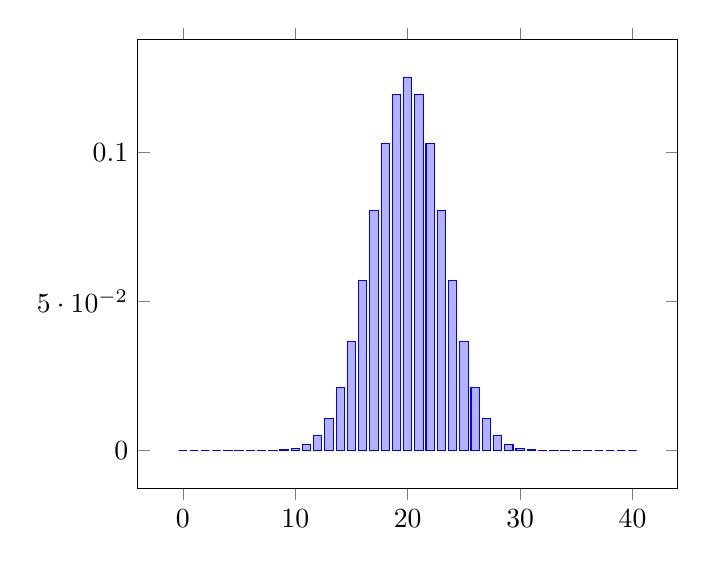
\begin{tikzpicture}
    \begin{axis} [ybar,bar width=3pt]
    \addplot coordinates {
        (0, 0.000000000000909)
        (1, 0.000000000036380)
        (2, 0.000000000709406)
        (3, 0.000000008985808)
        (4, 0.000000083118721)
        (5, 0.000000598454790)
        (6, 0.000003490986273)
        (7, 0.000016956219042)
        (8, 0.000069944403549)
        (9, 0.000248691212619)
        (10, 0.000770942759118)
        (11, 0.002102571161231)
        (12, 0.005081213639642)
        (13, 0.010944152454613)
        (14, 0.021106579733896)
        (15, 0.036584738205420)
        (16, 0.057163653445969)
        (17, 0.080701628394308)
        (18, 0.103118747392728)
        (19, 0.119400654875790)
        (20, 0.125370687619579)
        (21, 0.119400654875790)
        (22, 0.103118747392728)
        (23, 0.080701628394308)
        (24, 0.057163653445969)
        (25, 0.036584738205420)
        (26, 0.021106579733896)
        (27, 0.010944152454613)
        (28, 0.005081213639642)
        (29, 0.002102571161231)
        (30, 0.000770942759118)
        (31, 0.000248691212619)
        (32, 0.000069944403549)
        (33, 0.000016956219042)
        (34, 0.000003490986273)
        (35, 0.000000598454790)
        (36, 0.000000083118721)
        (37, 0.000000008985808)
        (38, 0.000000000709406)
        (39, 0.000000000036380)
        (40, 0.000000000000909)
    };
    \end{axis}
\end{tikzpicture}
\caption{Pravdepodobnostné rozdelenie počtu parametrov modelu pre \(\bar{k} = 20\), \(K = 40\) (rovnaká apriórna pravdepobnosť pre všetky modely)}
\label{priorprobs20_40}
\end{figure}

\begin{figure}[H]
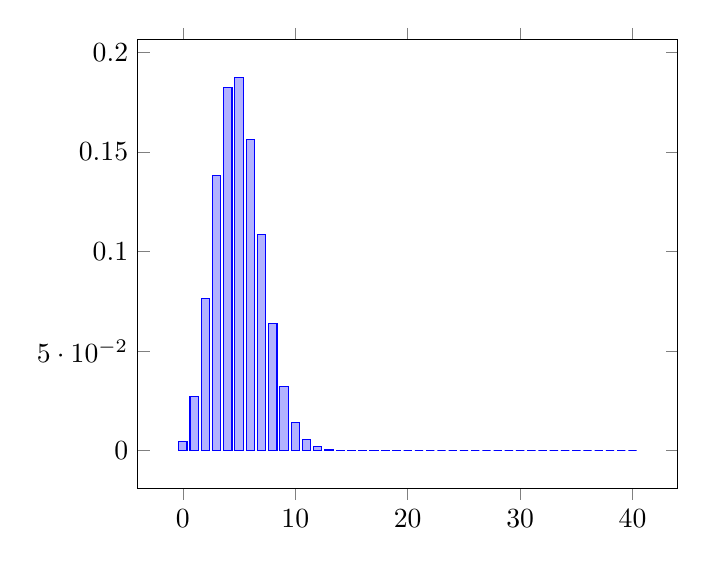
\begin{tikzpicture}

    \begin{axis} [ybar,bar width=3pt]
    \addplot coordinates {
        (0, 0.0047898522910280695238927073376089538215)
        (1, 0.0273705845201603972793868990720511646941)
        (2, 0.0762466283061611072024987834083731286228)
        (3, 0.1379700893159105656859964028626563958824)
        (4, 0.1823176180245961175430124967533629387617)
        (5, 0.1875266928252988518632804471053532324731)
        (6, 0.1562722440210823626749458981066709384322)
        (7, 0.1084338019738122493862420014920644462109)
        (8, 0.0638984904488536509248319816833827644587)
        (9, 0.0324563761010050327859843832811748143286)
        (10, 0.0143735379875879407118866026848991168663)
        (11, 0.0056000797354238737030263095562077069189)
        (12, 0.0019333608610391944410827891331905448169)
        (13, 0.0005948802649351367594424133677932786668)
        (14, 0.0001638955831964152346207769239683216256)
        (15, 0.0000405836682200647245674640650747733162)
        (16, 0.0000090588545134073045310418859088485988)
        (17, 0.0000018269958682502125610347398776411865)
        (18, 0.0000003334992457917054725548972049509189)
        (19, 0.0000000551652887775753427617234092572573)
        (20, 0.0000000082747933166363010840105296495040)
        (21, 0.0000000011258222199505173427959772713969)
        (22, 0.0000000001389001440198689936115356013957)
        (23, 0.0000000000155292086481841130332290368266)
        (24, 0.0000000000015714080179710112740529975861)
        (25, 0.0000000000001436715902144924531576991589)
        (26, 0.0000000000000118410651275680607835347202)
        (27, 0.0000000000000008771159353754118880724944)
        (28, 0.0000000000000000581760569381650769751543)
        (29, 0.0000000000000000034389787352609894172627)
        (30, 0.0000000000000000001801369813708137496838)
        (31, 0.0000000000000000000083012433811434902147)
        (32, 0.0000000000000000000003335321001352295176)
        (33, 0.0000000000000000000000115508952427785114)
        (34, 0.0000000000000000000000003397322130228974)
        (35, 0.0000000000000000000000000083199725638261)
        (36, 0.0000000000000000000000000001650788207108)
        (37, 0.0000000000000000000000000000025494798565)
        (38, 0.0000000000000000000000000000000287535322)
        (39, 0.0000000000000000000000000000000002106486)
        (40, 0.0000000000000000000000000000000000007523)
};
    \end{axis}
\end{tikzpicture}
\caption{Pravdepodobnostné rozdelenie počtu parametrov modelu pre \(\bar{k} = 5\), \(K = 40\)}
\label{priorprobs5_40}
\end{figure}

Aj keď volíme apriórne pravdepodobnosti nie pre modely, ale pre premenné,
pri ďalších výpočtoch budeme potrebovať aj apriórne pravdepodobnosti jednotlivých modelov.
Prístup, ktorý sme opísali vyššie, našťastie umožňuje ich jednoduchý výpočet: pre apriórnu pravdepodobnosť modelu \(M_i\) platí:

\[
p_{\text{prior}}(M_i) = \prod_{j = 1}^K \left( \frac{\bar{k}}{K} \right)^{I_{\beta_{j, i} \neq 0}} \left( 1 - \frac{\bar{k}}{K} \right)^{1 - I_{\beta_{j, i} \neq 0}},
\]

kde \( I_{\beta_{j, i} \neq 0} \) je indikátor zahrnutia \(j\)-tej premennej do modelu \(M_i\).
Uvedomme si, že apriórna pravdepobnosť modelu v tomto prípade závisí len od počtu premenných, ktoré v ňom vystupujú.
Ekvivalentný výpočet je:

\[
p_{\text{prior}}(M_i) = \left( \frac{\bar{k}}{K} \right)^{k_i} \left( 1 - \frac{\bar{k}}{K} \right)^{K - k_i},
\]

kde \( k_i) \) je počet premenných v modeli \( M_i \).

\subsubsection{Výpočet aposteriórnych pravdepodobností}

Aby sme mohli vyčísliť vzorce (\ref{posterior_expected_value}) a (\ref{posterior_inclusion_probability}) a získať tak odhady stredných hodnôt koeficientov a aposteriórne pravdepodobnosti zahrnutia premenných do modelu,
potrebujeme poznať aposteriórne pravdepodobnosti modelov.
Teoretické odvodenie výpočtu aposteriórnej pravdepodobnosti modelu budeme demonštrovať na modeli lineárnej regresie

\begin{equation} \label{linear_regression}
y = X \beta + \epsilon,
\end{equation}

kde \( \epsilon \sim N(0, \sigma^2 I) \).
Pri problematike selekcie premenných z množiny celkovo \(k\) potenciálnych premenných pracujeme s celkovo \(2^k\) modelmi zodpovedajúcimi každej možnej podmnožine k premenných,
vrátane modelu bez vysvetľujúcich premenných (t.j. len s interceptom) a plného modelu so všetkými \(k\) premennými.
Priestor všetkých modelov označme \(M = \{ M_1, M_2, \ldots, M_K \} \), \(K = 2^k\).

Každý model môžeme reprezentovať binárnym vektorom \(\gamma\) dĺžky \(k\), \( \gamma = (\gamma_1, \ldots, \gamma_k) \), kde \( \gamma_j \) je indikátor zahrnutia premennej \(X_j\) do modelu \(M_j\).
Pre model \(M_i\) predstavuje \( q_{\gamma} = \sum_{j=1}^k \gamma_j \) počet nenulových koeficientov, \(\beta_{\gamma} \) a \( X_{\gamma} \) predstavujú upravený vektor koeficientov a upravenú maticu dát pre model:

\begin{equation} \label{linear_regression_subset}
y = X_{\gamma} \beta_{\gamma} + \epsilon,
\end{equation}

v ktorom vystupujú len vysvetľujúce premenné dané vektorom \( \gamma \).
Exaktný výpočet aposteriórnych pravdepodobností si vyžaduje zadefinovanie hustôt jednolivých náhodných premenných vo vzorcoch (\ref{linear_regression}) a (\ref{linear_regression_subset}).

\begin{equation} \label{pdf_y}
    y | \beta, \sigma^2, M_i \sim N(X_{\gamma} \beta_{\gamma}, \sigma^2 I),
\end{equation}
\begin{equation} \label{pdf_beta}
    \beta_{\gamma} | \sigma^2, M_i \sim p(\beta_{\gamma} | \sigma^2, M_i),
\end{equation}
\[
    \sigma^2 | M_i \sim p(\sigma^2 | M_i),
\]
\begin{equation} \label{pdf_model}
    M_i \sim p(M_i).
\end{equation}

Hustota (\ref{pdf_y}) je ekvivalentná hustote, ktorú predpokladáme pri bežnej lineárnej regresii.
Hustota (\ref{pdf_beta}) predstavuje apriórne rozdelenie \( \beta_{\gamma}\), vektora nenulových prkov parametra \(\beta\) pre jednotlivé modely,
a (\ref{pdf_model}) predstavuje apriórnu pravdepodobnosť jednotlivých modelov (v našom prípade ide o pevné číslo).

Aposteriórne rozdelenie pravdepodobnosti modelu \(M_i\) možno vyjadriť vzťahom:

\[
    p(M_i | y) = \frac{m(y | M_i) p(M_i)}{\sum_{i = 1}^{K} m(y | M_i) p(M_i)},
\]

kde \( m(y | M_i) \) je marginálne rozdelenie dát pre model \(M_i\) dané vzťahom:

\begin{equation} \label{marginal_y}
    m(y | M_i) = \int \int p(y | \beta_{\gamma}, \sigma^2, M_i) p(\beta_{\gamma} | \sigma^2, M_i) p(\sigma^2 | M_i) d\beta_{\gamma} d\sigma^2.
\end{equation}

Aposteriórne rozdelenie pravdepodobnosti \( p(M_i | y) \) reprezentuje mieru neistoty o modeli \(M_i\) po pozorovaní dát \(y\).

Enumerácia integrálu v (\ref{marginal_y}) býva často náročná úloha.
V prípade lineárnej regresie existujú voľby apriórnych rozdelení, ktoré vedú k analytickému vyjadreniu integrálu (\ref{marginal_y}) \cite{mcculloch}.
V našej práci budeme aposteriórne pravdepodobnosti modelov aproximovať vzťahom prevzatým z \cite{jamespress},
ktorý okrem lineárnej regresie platí aj pre zovšeobecnené linerálne modely (angl. \emph{generalized linear models}):

\begin{equation} \label{posterior_model_approximation}
        p(M_i | y) = \frac{p(M_i) e^{-\frac{1}{2}BIC(M_i)}}{\sum_{i = 1}^{K} p(M_i) e^{-\frac{1}{2}BIC(M_i)}}.
\end{equation}

\(BIC\) predstavuje bayesovské informačné kritérium (angl. \emph{Bayesian infomation criterion}), ktoré je definované nasledovne:

\[
    BIC(M_i) = m \ln{n} - 2 \ln{\hat{L}},
\]

kde \( m \) je počet parametrov vystupujúcich v modeli, \(n\) je počet dát,
a \(\hat{L}\) je maximum pravdepodobnostnej funkcie modelu pre dané dáta \(X_{\gamma}\) a \(y\).
\(BIC\) je ľahko vypočítateľná hodnota a umožní nám ľahkú a presnú aproximáciu aposteriórnych pravdepodobností jednotlivých modelov.

\subsubsection{Implementácia metódy \emph{BACE}}

V ideálnom svete by sme pre pre \(k\) potenciálnych vysvetľujúcich premenných vyčíslili všetkých \(2^k\) modelov,
čo by nám poskytlo presný výsledok pre aposteriórne pravdepodobnosti modelov a posteriórne pravdepodobnosti zahrnutia premenných (pri predpodkladaných apriórnych pravdepodobnostiach).
V praxi býva \(2^k\) príliš veľké na takúto \emph{exhaustívnu} enumeráciu – v pôvodnom článku Sala-i-Martina pracovali autori s \(k = 32\) premennými, my máme premenných \(74\).

Riešením je odhadnúť len časť z množiny \(2^k\) modelov, pričom konkrétnych implementácií nájdeme v literatúre niekoľko.
V článku \cite{sala-i-martin} autori navrhli a použili heuristiku, ktorá po mnoho iterácií generuje modely obsahujúce náhodnú množinu vysvetľujúcich premenných,
až kým odhad strednej hodnoty neskonverguje (podľa nejakého vopred stanoveného kritéria).
Apriórnou informáciou, ktorú pri tomto prístupe treba zvoliť, sú apriórne pravdepodobnosti jednotlivých modelov.
Podobne ako v tejto práci, aj my pri implementácii tejto metódy apriórne pravdepodobnosti modelov spočítame pomocou apriórnych pravdepodobností zahrnutia premenných,
ktorú zvolíme ako \(\bar{k}/K\) podľa očakávaného počtu vysvetľujúcich premenných \(\bar{k}\) v „skutočnom“ modeli.
Odhad strednej hodnoty parametra \(\beta\) spočítame vzorcom (\ref{posterior_expected_value}),
pričom aposteriórne pravdepodobnosti jednotlivých modelov odhadneme pomocou aproximácie (\ref{posterior_model_approximation}) využívajúcej hodnoty \emph{BIC} pre jednotlivé modely.

V práci \cite{ondrusekova} autorka použila prístup, pri ktorom kompletne enumerovala len časť modelov – tie so \(4\), \(5\), či \(6\) premennými.
V našej práci implementujeme aj túto verziu metódy \emph{BACE}, pričom ale budeme enumerovať len modely s \(5\) premennými (vychádzajúc z očakavaného počtu premenných \(\bar{k} = 5\)).
Aproximácia aposteriórnych pravdepodobností modelov, odhady strednej hodnoty parametra \(\beta\) a aposteriórnych pravdepodobností zahrnutia jednotlivých premenných počítame pomocou vzorcov
(\ref{posterior_model_approximation}), (\ref{posterior_expected_value}) a (\ref{posterior_inclusion_probability}).